This chapter is dedicated to elaborate the various aspects which are related to evaluation process. Primarily it is focused on the implementation and execution details of the NIST statistical test suite, followed by the test invocation examples. Along with the NIST suite, the Initial Random String Test and the results are also elaborated here, along with the interpretation of the results. Then, the various test results and their interpretations along with the possible conclusions are derived towards the latter half of the chapter.

\section{Initial Random String Test - Observations}

As discussed previously, the evaluation on this test is two fold. The results and the interpretation are as elaborated in the subsections below. The results enumerated here are for 1000 samples.

\subsection{Visual Inspection}

The visual inspection on the images was done primarily taking the following concerns into account.

\begin{enumerate}
    \item Perceived Similarity with the TV noise image
    \item Absence of any obvious patterns
    \item Plain white/black patches which are obviously large
\end{enumerate}

The results and the interpretation of the visual inspection could be itemised per each appended digit up to \nth{8} image, as below (Figure \ref{fig:4_seed_1}).

\begin{itemize}
    \item \textbf{1 Digit} - When it is only one digit, except for '$5$', all other digits demonstrated a pattern with alternating lines. The image generated by the seed $0.8$ is given in the figure below (Figure \ref{fig:4_seed_1}).
    
    \begin{figure}[h!]
        
\includegraphics[width=0.6\textwidth]{irst/0001.png}
        \centering
        \caption{Bitmap of Random String - 1 Digit Seed}
        \label{fig:4_seed_1}
    \end{figure}
    
    \item \textbf{2-4 Digits} - A relatively small patch which appears to be uneven is repeated over the whole image. Bitmap generated by  the seed with 2-3 digit appears to demonstrate some check/diagonal pattern. The bitmap generated with 3-digit seed is as depicted in figure \ref{fig:4_seed_3}
    
    \begin{figure}[h!]
        
\includegraphics[width=0.6\textwidth]{irst/0003.png}
        \centering
        \caption{Bitmap of Random String - 3 Digit Seed}
        \label{fig:4_seed_3}
    \end{figure}
    
    \item \textbf{5-6 Digits} - A relatively large patch which appears to be uneven is repeated over the whole image. Since the patch is large, the number of times that the pattern is repeated has become lesser. Pattern still appears to be somewhat diagonal. Figure \ref{fig:4_seed_5} indicates the bitmap generated with a seed of 5 digits.
    
    \begin{figure}[h!]
        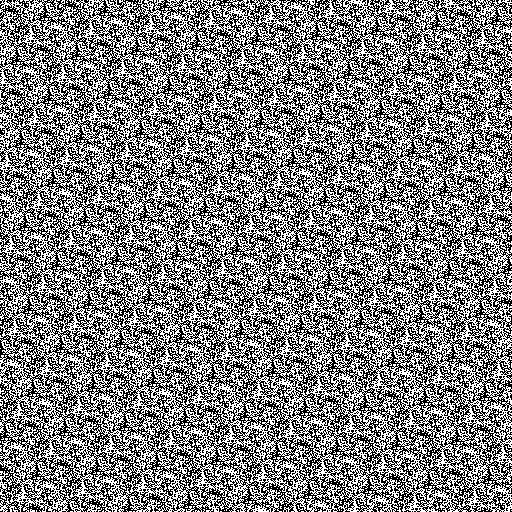
\includegraphics[width=0.6\textwidth]{irst/0005.png}
        \centering
        \caption{Bitmap of Random String - 5 Digit Seed}
        \label{fig:4_seed_5}
    \end{figure}
    
    \item \textbf{7 Digits} - The pattern has become much less obvious in the bitmap generated with 7 digits seed. Figure \ref{fig:4_seed_7} indicates the bitmap generated with a seed of 7 digits. However, upon closer examination, some pattern could be observed. This gets obvious when the dimensions of the bitmap are increased.
    
    \begin{figure}[h!]
        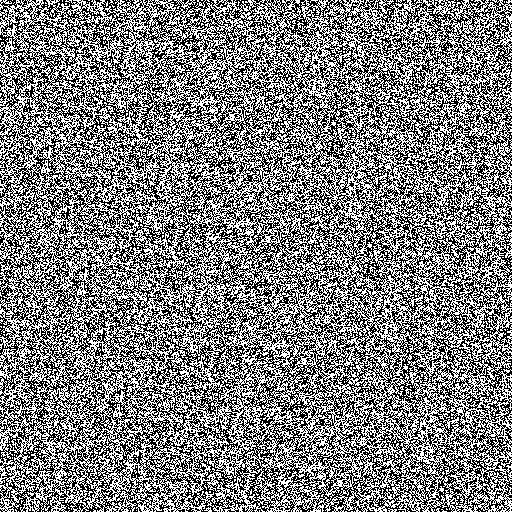
\includegraphics[width=0.6\textwidth]{irst/0007.png}
        \centering
        \caption{Bitmap of Random String - 7 Digit Seed}
        \label{fig:4_seed_7}
    \end{figure}
    
    \item \textbf{8 Digits and above} - No obvious patterns are visible beyond 8 digits. However, it has not tested if there exists a pattern as the number of bits generated by the generator is increased. This is to be further tested in the next iterations of development. Figure \ref{fig:4_seed_8} indicates the bitmap generated with a seed of 8 digits, while figure \ref{fig:4_seed_10} depicts the bitmap of the bit string generated with 10 digit seed.
    
    \begin{figure}[h!]
        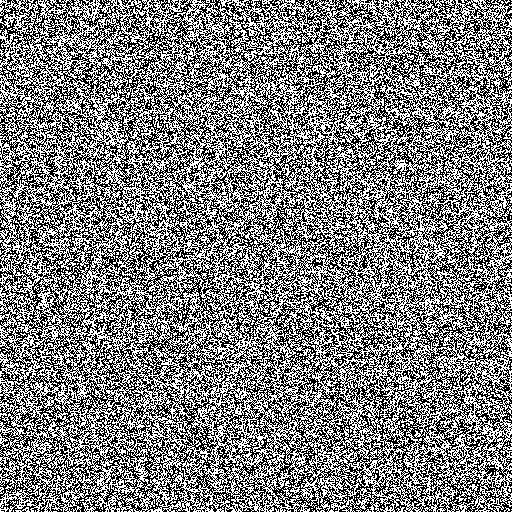
\includegraphics[width=0.6\textwidth]{irst/0008.png}
        \centering
        \caption{Bitmap of Random String - 8 Digit Seed}
        \label{fig:4_seed_8}
    \end{figure}
    
    \begin{figure}[h!]
        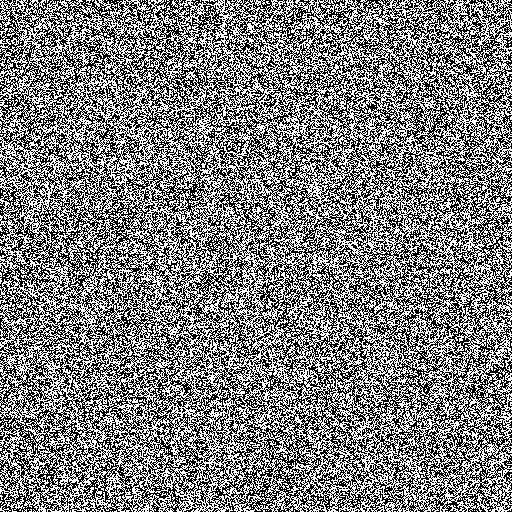
\includegraphics[width=0.6\textwidth]{irst/0010.png}
        \centering
        \caption{Bitmap of Random String - 10 Digit Seed}
        \label{fig:4_seed_10}
    \end{figure}
\end{itemize}

\subsection{Statistical Testing on Bitmaps}

Then, each generated bitmap is compared against the bitmap $B$ of TV noise. For this comparison, the MSE and the SSIM values for each of the sample against $B$ were computed and the variation of the MSE values are plotted against the sample number, into a two dimensional line chart as depicted in figure \ref{fig:4_mse_var_init_samples}.

\begin{figure}[h!]
    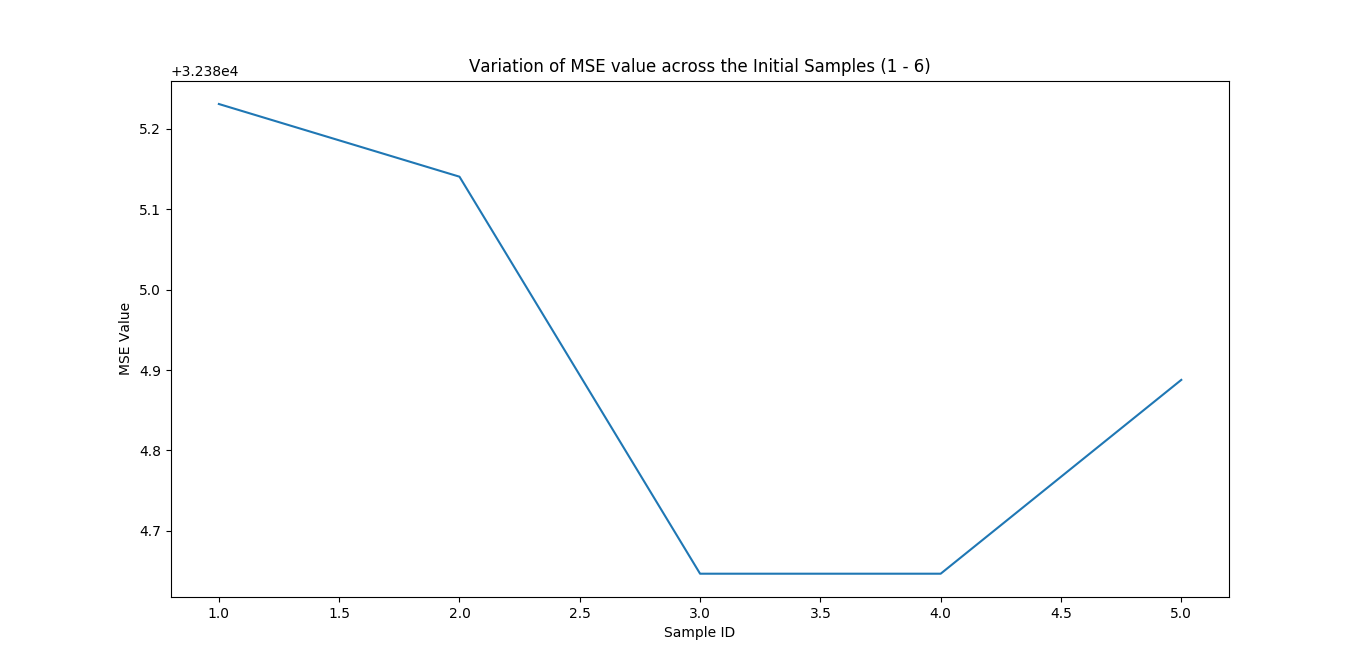
\includegraphics[width=1.0\textwidth]{images/mse_init_1_6.png}
    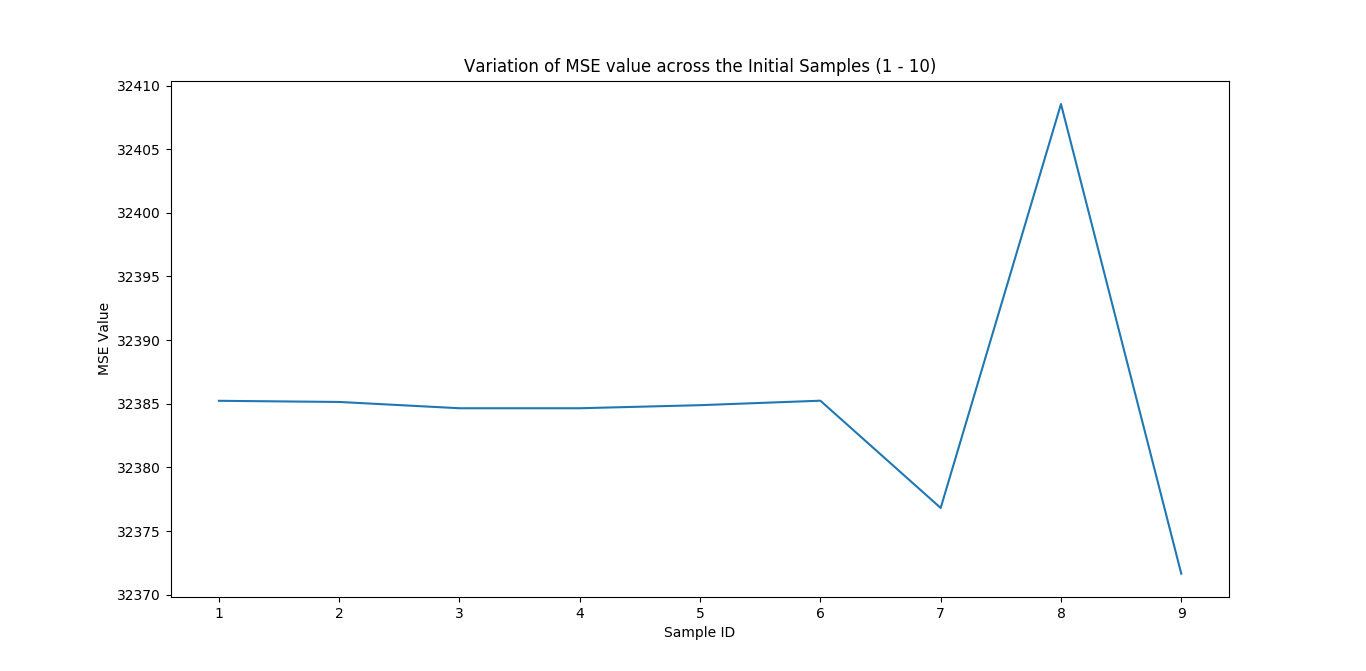
\includegraphics[width=1.0\textwidth]{images/mse_init_1_10.png}
    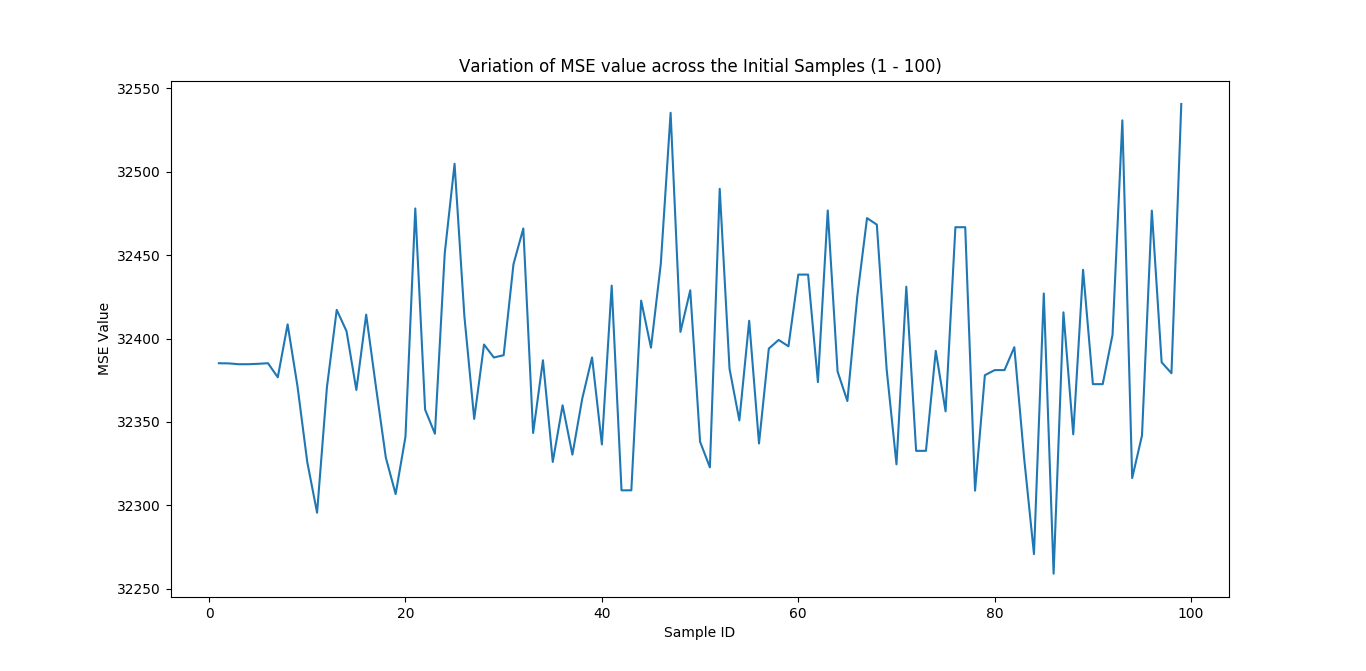
\includegraphics[width=1.0\textwidth]{images/mse_init_1_100.png}
    \centering
    \caption{Variation of the MSE of the Samples in Initial Random String Test}
    \label{fig:4_mse_var_init_samples}
\end{figure}

When these are observed, it is quite evident that the variation of the MSE for the first 6 samples are not that high. Yet, beyond that point, the MSE starts to vary quite rapidly and the variation is not demonstrating any patterns. This is visible in the graphs below (figures )

% \begin{figure}[h!]
%     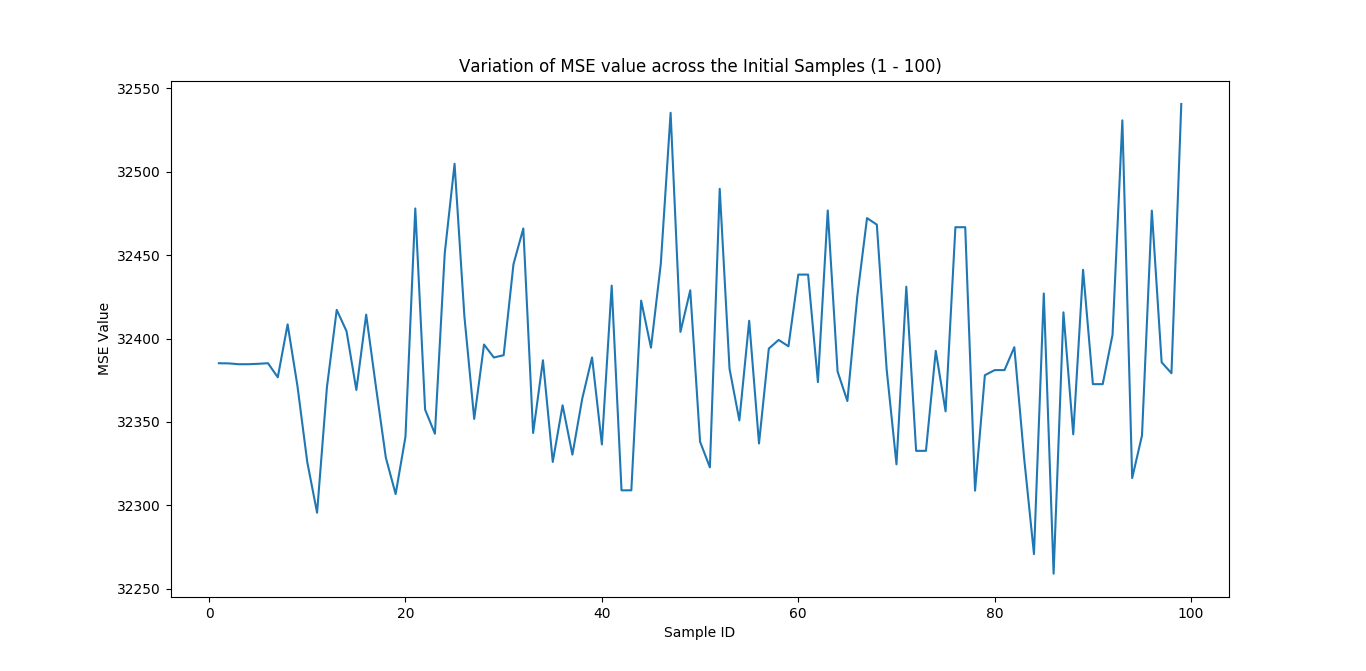
\includegraphics[width=1.0\textwidth]{images/mse_init_1_100.png}
%     \centering
%     \caption{Variation of the MSE of the Samples in Initial Random String Test (Samples 1 - 100)}
%     \label{fig:4_mse_1_6}
% \end{figure}

These observations are falling in line with the observations of the visual inspection outlined above. The observations were quite similar when the same test was conducted on other samples of randomly chosen strings. Further, each of the bit strings was tested with the NIST suite and a summary report for each random string tested is generated. The test reports correspond to sample $0001$ and $0500$ are attached as appendix \ref{adx:nist_summary_sample_init_0001} and appendix \ref{adx:nist_summary_sample_init_0500} respectively. The test results were summarised as follows.

\begin{itemize}
    \item Total number of instances, passed and skipped of each instance was summarised as mentioned below.
    
    \begin{code}
        \begin{minted}[breaklines,tabsize=2]{json}
        {
            "_id" : "SAMPLE_0001",
            "passed" : 6,
            "total" : 188,
            "passRate" : 0.0319148936170213
        }
        \end{minted}
    \end{code}
    
    \item Then, the passRate was plotted against the sample id in a 2D plot (figure \ref{fig:4_nist_init_samples_1_500}). 
\end{itemize}

\begin{figure}[h!]
    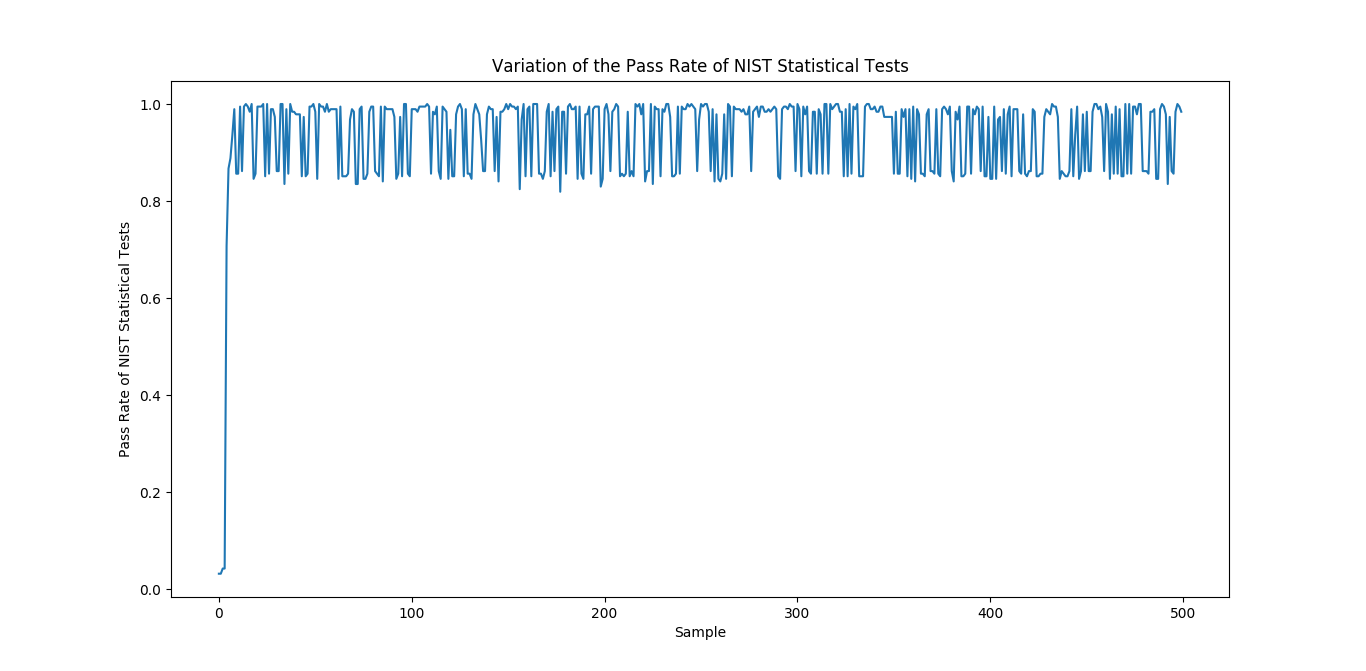
\includegraphics[width=1.0\textwidth]{images/pass_rates_nist_init_sample_1_500.png}
    \centering
    \caption{Variation of the Pass Rate of NIST Test Suite of Samples in Initial Random String Test (Samples 1 - 500)}
    \label{fig:4_nist_init_samples_1_500}
\end{figure}

Upon closer observation, it is evident that the initial samples are showing very low pass rates and beyond sample bearing the ID 6, the pass rates of the tests exceed 80\% of pass rate and settle to vary almost linearly around 90\%. Test which are dropping the pass rate close to 80\% are the tests that which the instances Random Excursion Test and Random Excursion Test (Variant) were skipped due to the inadequate number of cycles in the random walk of each bit string. This could be better observed in the graphs below (figure \ref{fig:4_nist_init_samples})

\begin{figure}[h!]
    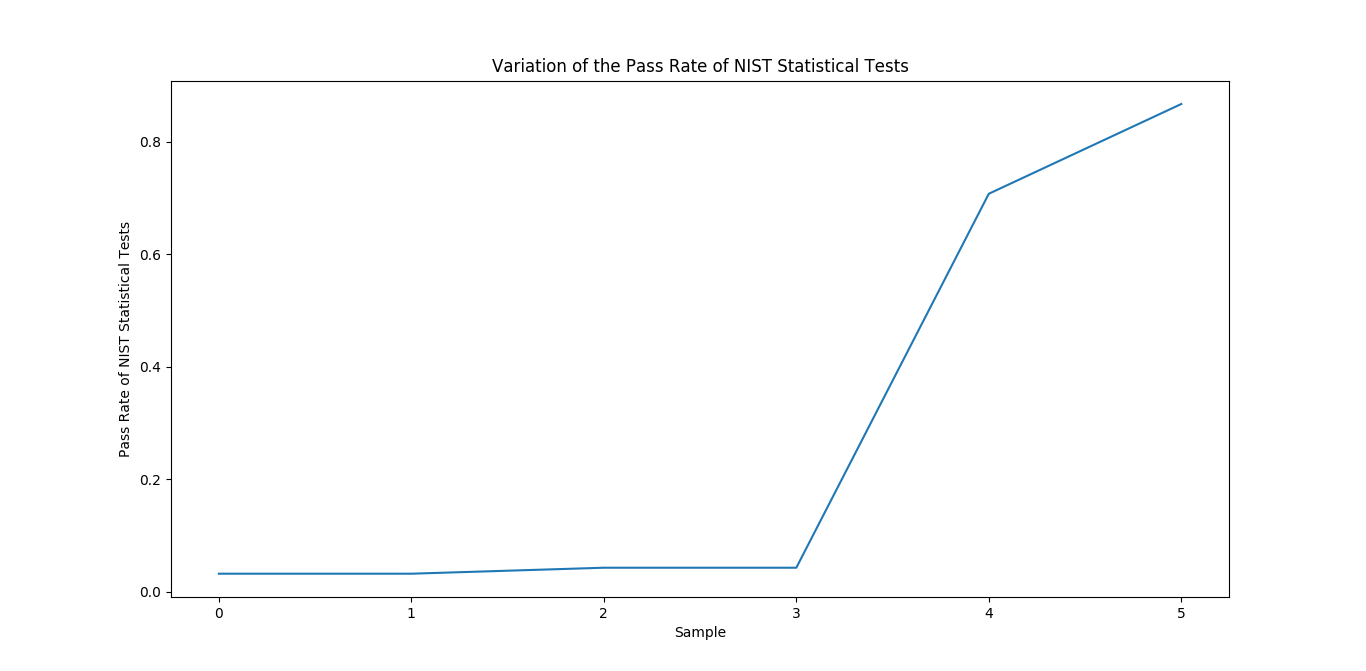
\includegraphics[width=1.0\textwidth]{images/pass_rates_nist_init_sample_1_6.png}
    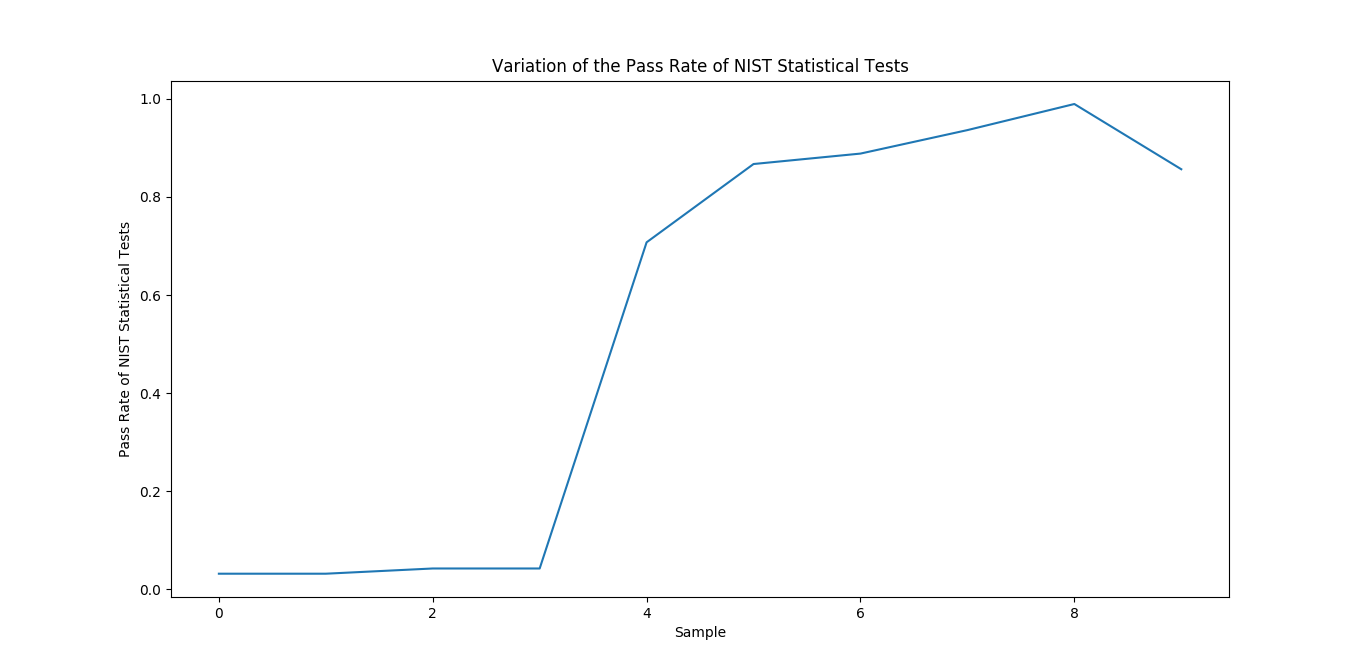
\includegraphics[width=1.0\textwidth]{images/pass_rates_nist_init_sample_1_10.png}
    \centering
    \caption{Variation of the Pass Rate of NIST Test Suite of Samples in Initial Random String Test (Samples 1 - 6)}
    \label{fig:4_nist_init_samples}
\end{figure}

\subsection{Performance during Testing}

For generating $10^6$ bits, the processing time has demonstrated variations which are as summarised and enumerated below, in the second itemised list. The generation timings were measured in a device with the following configuration.

\begin{itemize}
    \item \textbf{Processor} - Intel Core i5-6400 CPU @ 2.70GHz $\times$ 4
    \item \textbf{RAM} - 7.7GiB
    \item \textbf{Graphics} - Intel HD Graphics 530 (Skylake GT2)
    \item \textbf{OS} - Ubuntu 16.04 LTS
\end{itemize}

\subsubsection{Observations}
\begin{itemize}
    \item During the earliest stage (i.e. between 1-10 digits), the generation time was well below a second.
    
    \item Up to 20 digits of seed, the generation time of the random string was close to, but less than a second.
    
    \item Between 20 to 500 digits, the generation time was rapidly increasing and the average generation time lies around five to seven seconds.
    
    \item Above 500 digits, the generation becomes quite slow, and towards the latter stage, the generation time has exceeded 10 seconds.
\end{itemize}

As per the observation enumerated above, the period for repetitions which could cause obvious patterns, rises as the seed length grows. So, longer the seed, better the generation would be. Nevertheless, at the same time, the processing time complexity also rise as the number of digits in the seed is increased. It has a time complexity of $O(n \cdot l)$, where $n$ is the number of digits and $l$ is the length of the bit stream. Hence, the optimum combination of $n$ and $l$ is dependent on the requirement. However, the test combination used during the study (i.e. $n=20$ and $l=10^6$) appeared to be sufficiently performant in terms of volume and statistical quality.

\section{Visual Inspections}

Further, the data sequences chosen were visually inspected by plotting them on graphs against the timestamp they were obtained. This was conducted for the both IDLE and WORKING systems. Obtained plots are as graphically depicted below. Figure \ref{fig:4_plt_int_counts} depicts the variation of the total number of hardware interrupts count while figure \ref{fig:4_plt_sw_int_counts} and \ref{fig:4_plt_int_sw_int_ratios} depicts the variations of total number of software counts and the ratio between hardware and software counts respectively.

\begin{figure}[h!]
    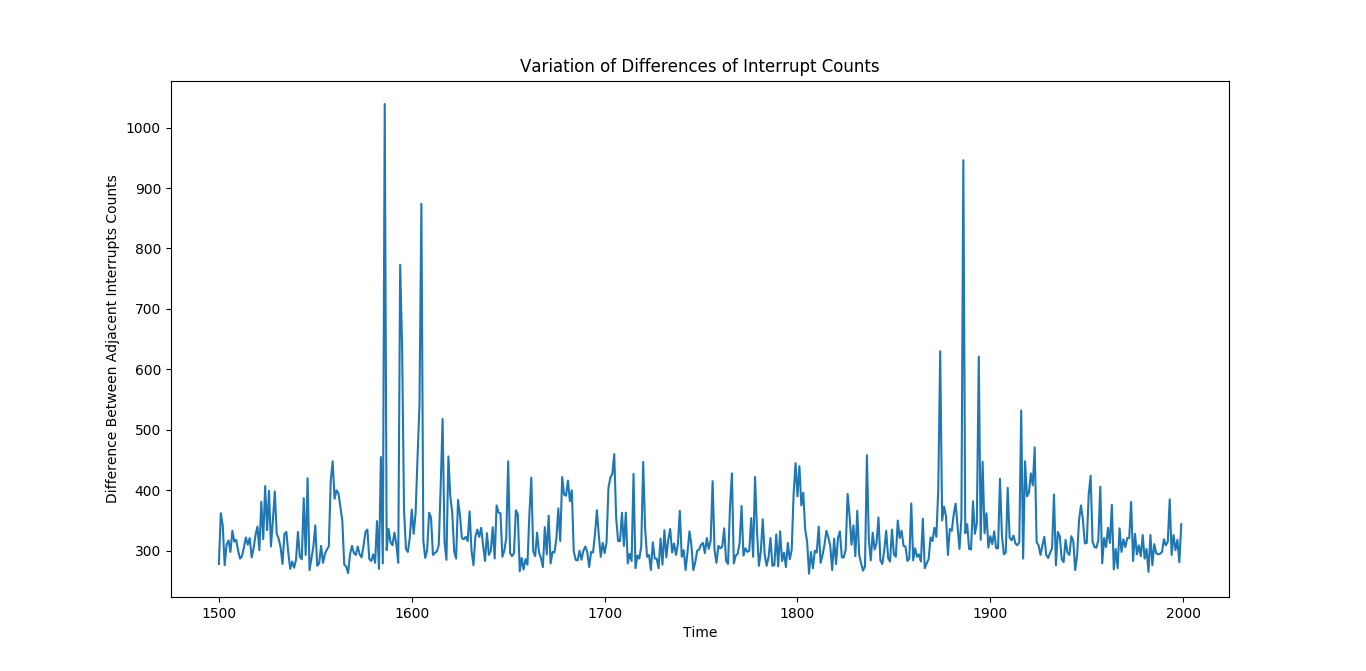
\includegraphics[width=1.0\textwidth]{images/PLT_ADJ_INTERRUPTS_DIFFERENCES_IDLE_1500_500.png}
    \centering
    \caption{Variation of the Total Hardware Interrupts Count (Between \nth{1500} and \nth{2000} seconds)}
    \label{fig:4_plt_int_counts}
\end{figure}

\begin{figure}[h!]
    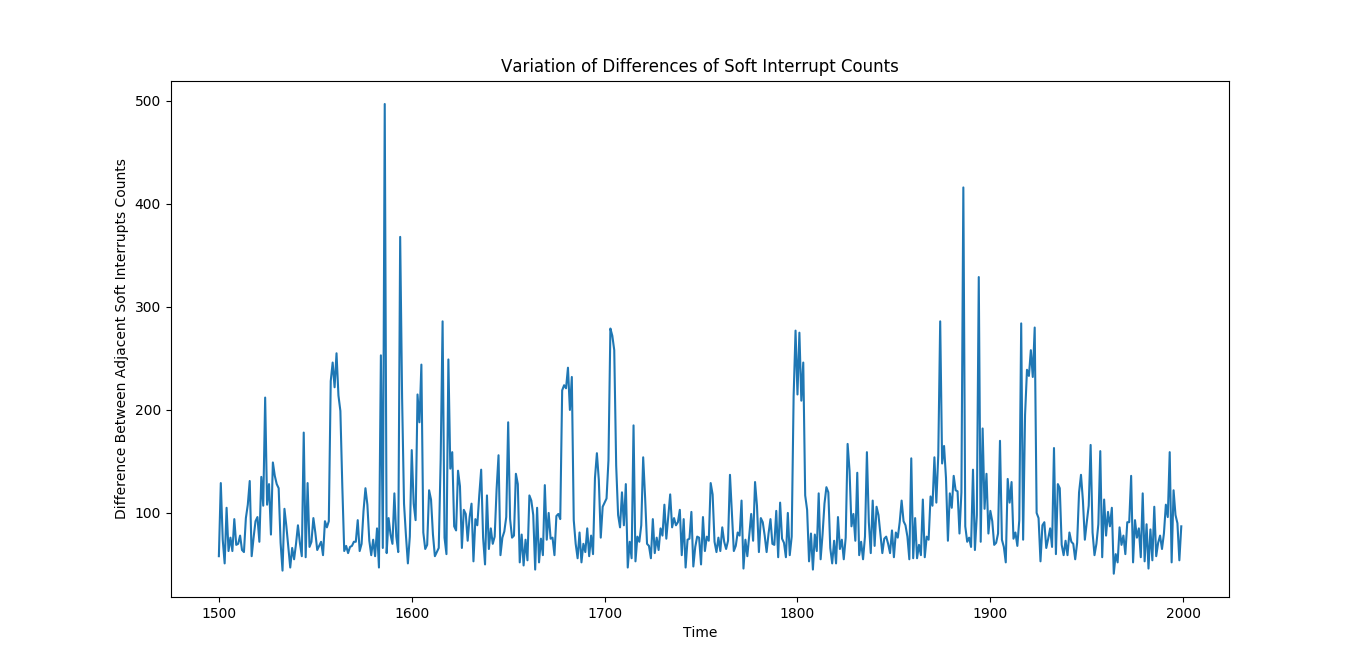
\includegraphics[width=1.0\textwidth]{images/PLT_ADJ_SOFT_INTERRUPTS_DIFFERENCES_IDLE_1500_500.png}
    \centering
    \caption{Variation of the Total Software Interrupts Count (Between \nth{1500} and \nth{2000} seconds)}
    \label{fig:4_plt_sw_int_counts}
\end{figure}

\begin{figure}[h!]
    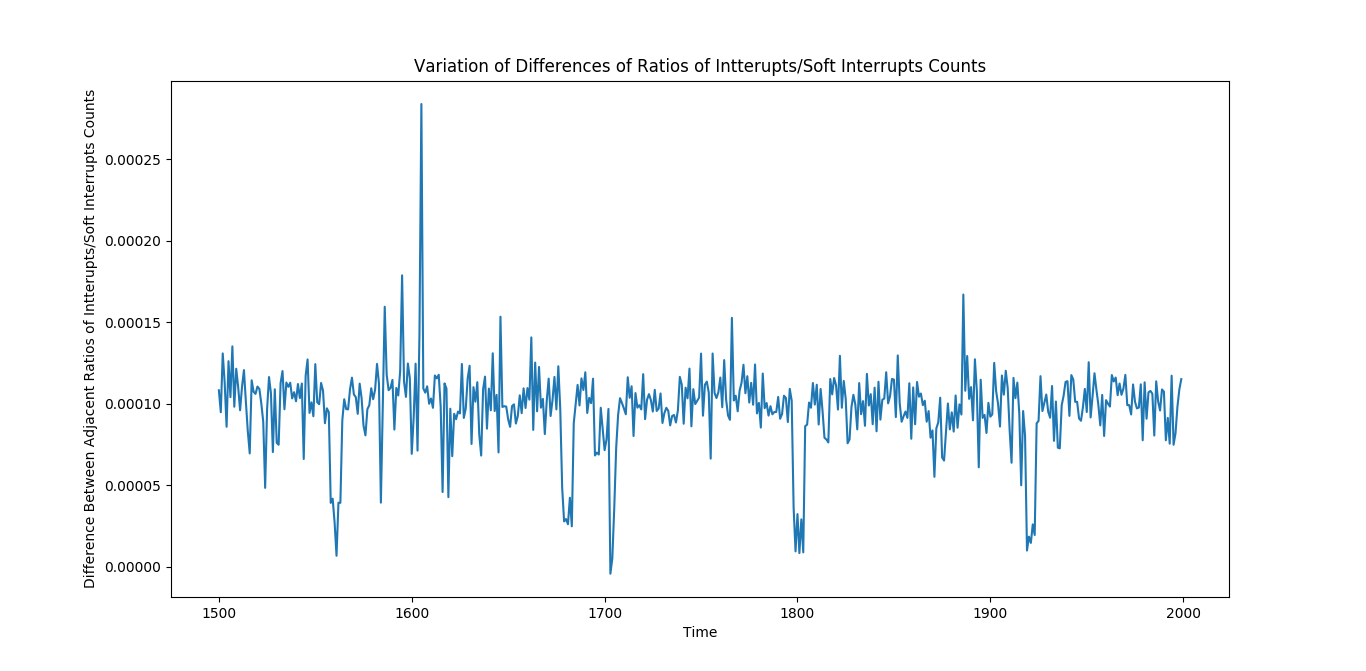
\includegraphics[width=1.0\textwidth]{images/PLT_ADJ_INTERRUPTS_RATIOS_DIFFERENCES_IDLE_1500_500.png}
    \centering
    \caption{Variation of the Ratio between the Hardware and Software Interrupts Count (Between \nth{1500} and \nth{2000} seconds)}
    \label{fig:4_plt_int_sw_int_ratios}
\end{figure}

\section{Test Results}

Afterwards, the data sequences were used as seeds for the generator and $10^6$ bit long bit sequences were generated from each seed pair. Then each of the bit string generated was tested with the NIST statistical test suite. For these tests, only a sample of observations were used from each of the IDLE and WORKING system. This constraint was imposed due to the long time which was consumed. For each bit string of $10^6$ bits, it takes little over 1 minute to complete the entire test suite and each test produces a test summary, which is as given in appendix \ref{adx:nist_summary_sample_idle}.

For bench marking, two of the previously discussed algorithms were used. Mersenne Twister (MT19937) and Xoroshiro128+ was used for bench marking and LFSR was purposely dropped from the benchmark due to the fact that the generator is already outdated. From each of MT and Xoroshiro128+, 1000 samples of random strings were generated and each of these were statistically tested using the NIST test suite.

\begin{table}[h!]
    \centering
    \begin{tabular}{|l|c|}
        \hline
        \multicolumn{1}{|c|}{\textbf{Test Name}} & \textbf{Number of Instances} \\ \hline
        Frequency & 1 \\ \hline
        Block Frequency & 1 \\ \hline
        Cumulative Sums & 2 \\ \hline
        Runs & 1 \\ \hline
        Longest Run & 1 \\ \hline
        Rank & 1 \\ \hline
        Spectral (DFT) & 1 \\ \hline
        Non Overlapping Template & 148 \\ \hline
        Overlapping Template & 1 \\ \hline
        Universal & 1 \\ \hline
        Approximate Entropy & 1 \\ \hline
        Random Excursion & 8 \\ \hline
        Random Excursion (Variant) & 18 \\ \hline
        Serial & 2 \\ \hline
        Linear Complexity & 1 \\ \hline
        \textbf{Total Number of Instances} & \textbf{188} \\ \hline
    \end{tabular}
    \caption{Total number of Instances per Test Class}
    \label{tbl:5_nist_total_instances}
\end{table}

The test suite executes multiple instances of each tests, selected from the entire set. Out of the all of 15 tests, Random Excursion Test and Random Excursion (Variant) Test was not executed on approximately 45\% of the entire samples which were tested. This was due to the absence of sufficient number of random walks in the bit strings which were skipped. All of the other tests were executed. There are a total of 188 test instances from all tests, that which the number of instances executed for each test is as tabulated below (table \ref{tbl:5_nist_total_instances}).

The test summary was used to summarise the test results for each of the systems. Similar to the previous case of Initial Random String Test, here also the pass counts were summarised for each sample tested as follows.

\begin{code}
    \begin{minted}[breaklines,tabsize=2]{json}
    {
        "_id" : "2090775_1536805",
        "passed" : 161,
        "total" : 188,
        "passRate" : 0.856382978723404
    }
    \end{minted}
\end{code}

Then, these summaries were plotted on 2D line graphs against their index in the sequence. The variation of the pass rates of the tests conducted for the proposed algorithm are as depicted below in figure \ref{fig:4_nist_pass_rates}. The top most graph plots the variations of the proposed algorithm executed on the idle system. The graph at the middle plots the variation of the pass rates of MT and the bottom most graph plots the same data that are of the Xoroshiro128+.

\begin{figure}[h!]
    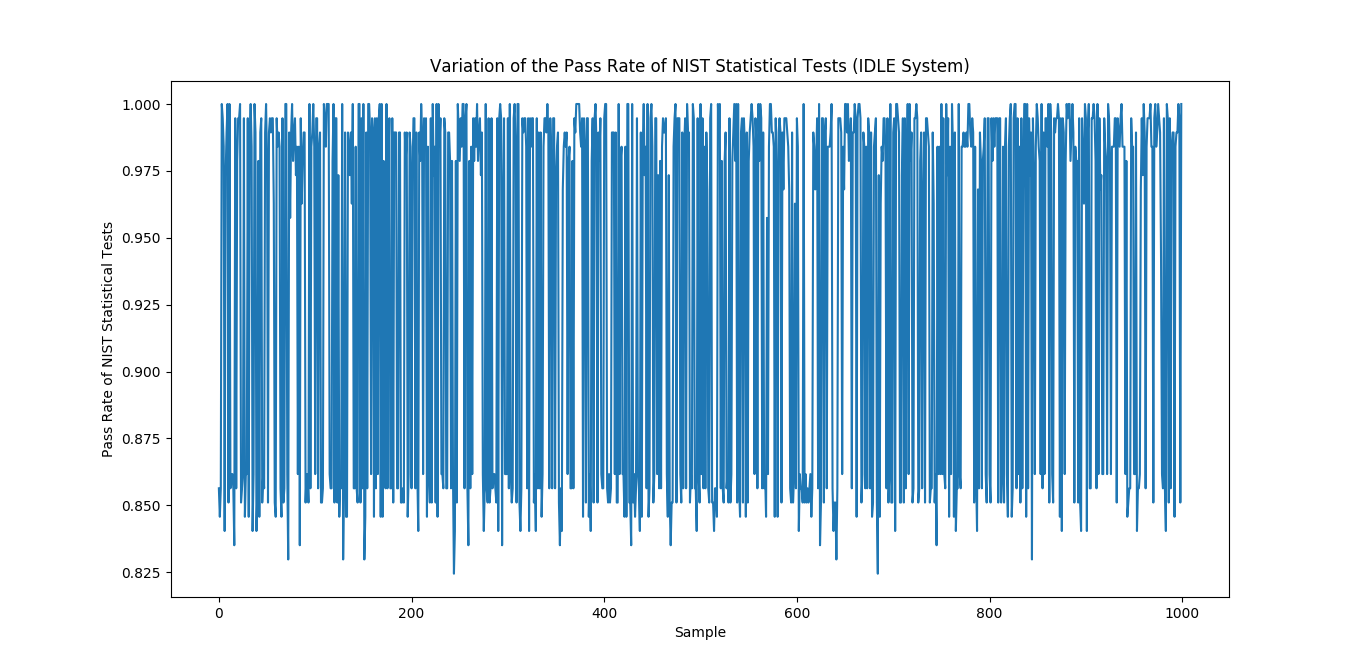
\includegraphics[width=1.0\textwidth]{images/nist_pass_rate_idle.png}
    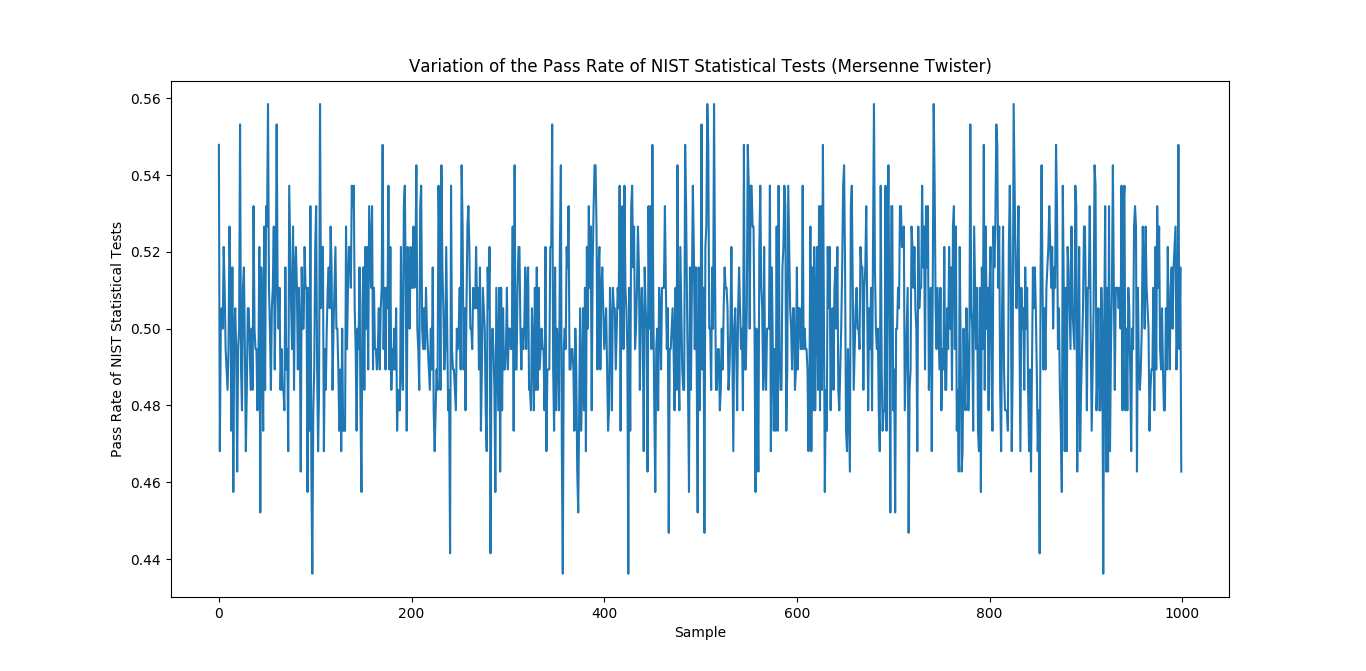
\includegraphics[width=1.0\textwidth]{images/nist_pass_rate_mt.png}
    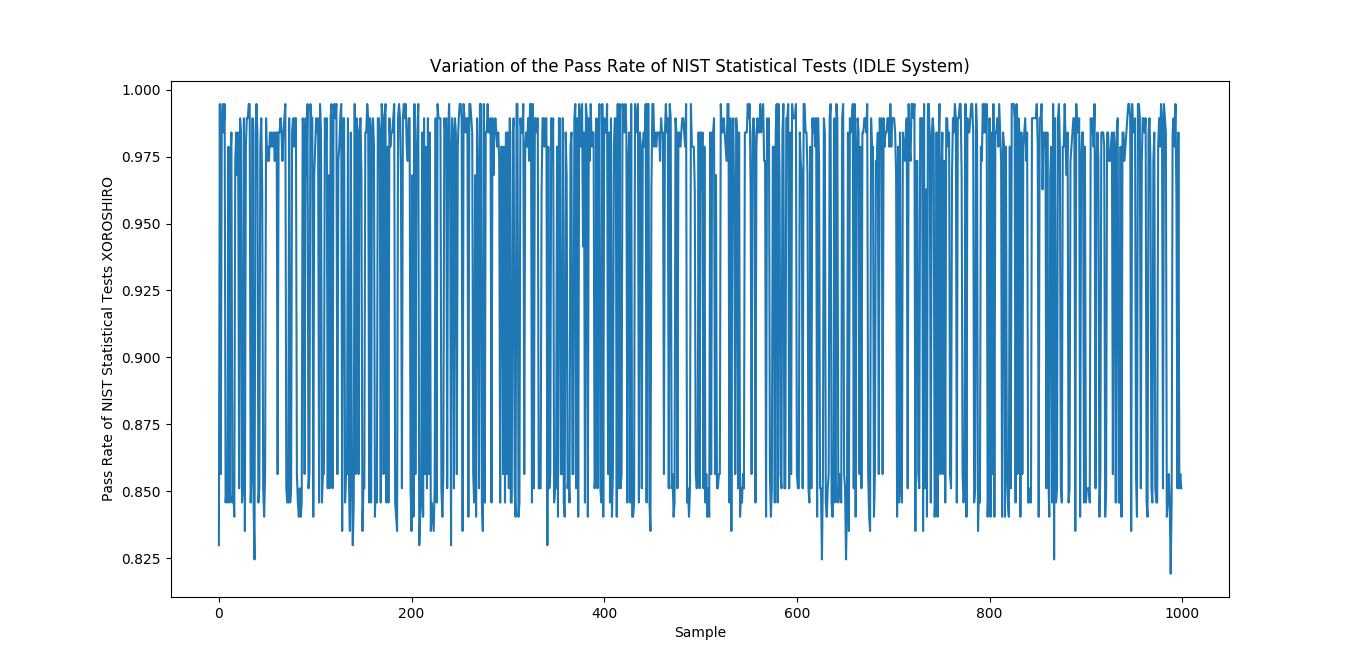
\includegraphics[width=1.0\textwidth]{images/nist_pass_rate_xoroshiro.png}
    \centering
    \caption{Variation of the Pass Rate of NIST Test Suite for Proposed Algorithm, MT and Xoroshiro128+}
    \label{fig:4_nist_pass_rates}
\end{figure}

\subsubsection{Interpretation}

Upon close examination it is evident that the pass rates of the random strings generated by the proposed algorithm are much higher compared to the pass rates of the bit strings generated by the Mersenne Twister. The proposed algorithm shows pass rates between 82\% and 100\% with much large variation, while Mersenne Twister demonstrates results which are between 44\% and 56\% with comparatively less variation. For the case of Xoroshiro128+, the pass rates vary between 82\% and 99.9\%, with the lower bound of variation is mostly close to 85\%. This is almost similar and close to that of the proposed algorithm.

\section{Statistical Summarising of Test Results}

Then the sequences of pass rates were summarised using the mean, variance and standard deviation for each sequence. These measures were obtained for each of the system considered and they are as tabulated below (table \ref{tbl:5_stat_summary}).

\begin{table}[h!]
    \centering
    \scriptsize
    \begin{tabular}{|l|r|r|r|}
        \hline
        \textbf{System} & \textbf{Mersenne Twister} & \textbf{Xoroshiro128+} & \textbf{FloatRAND (Idle)} \\ \hline
        \textbf{Mean} & 0.501771 & 0.935840 & 0.934809 \\ \hline
        \textbf{Variance} & 0.000407 & 0.004422 & 0.004563 \\ \hline
        \textbf{Standard Deviation} & 0.021690 & 0.066500 & 0.067552 \\ \hline
    \end{tabular}
    \caption{Summary of Statistical Measures}
    \label{tbl:5_stat_summary}
\end{table}

\subsubsection{Interpretation}

Since the mean values for proposed algorithm and MT are $0.934809 $ and $0.501771$ respectively, the higher mean of the proposed algorithm, suggests that the average statistical quality is much higher in the proposed algorithm than the typical MT. The difference is roughly about 43\% between the two. However, the proposed algorithm demonstrates much higher standard deviation, which is almost 5\% more than that of the MT. This suggests that MT demonstrates more consistency than the proposed algorithm in terms of the statistical quality. These properties are further highlighted by the graphs provided in figure \ref{fig:4_nist_pass_rates}.

Compared to the case of MT vs. proposed algorithm, the results of the comparison of Xoroshiro128+ and the proposed algorithm, are much closer. The mean values of the pass rates of Xoroshiro128+ and the proposed algorithm are $0.935840$ and $0.934809$ respectively, where the Xoroshiro128+ has demonstrated slightly better pass rates which is about 0.001\%. When the standard deviations are compared, the standard deviation of the pass rates of Xoroshiro128+ is about 0.001\% lower than that of the proposed algorithm. Hence, it could be concluded that the Xoroshiro128+ is slightly more consistent in terms of the pass rates, than the proposed algorithm. Yet, the differences are at small scales.